\section{Corrida de prueba}

\begin{itemize}
  \item Opciones al correr el servicio de localización.
\end{itemize}
\begin{center}
  \small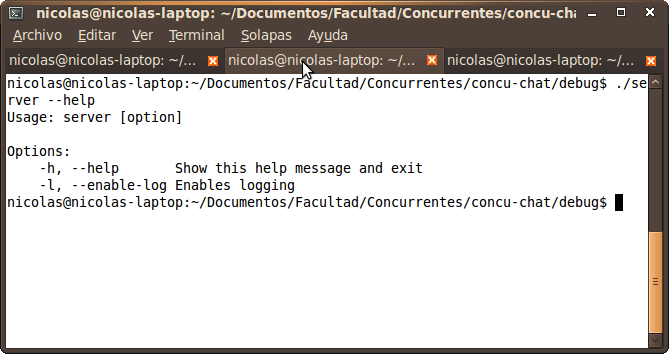
\includegraphics[scale=0.65]{./Images/AyudaServer}
\end{center}

\begin{itemize}
  \item Opciones al correr un cliente.
\end{itemize}
\begin{center}
  \small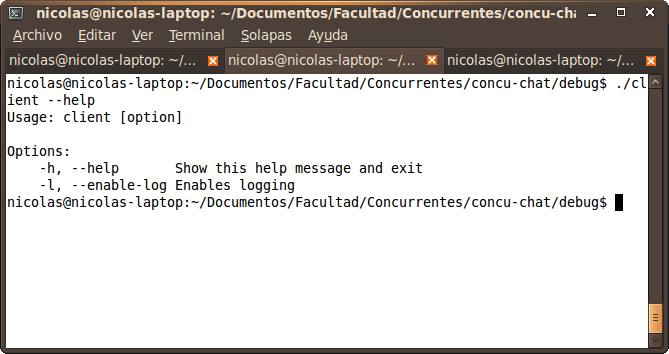
\includegraphics[scale=0.65]{./Images/AyudaCliente}
\end{center}

\begin{itemize}
  \item Correr servicio de localización.
\end{itemize}
\begin{center}
  \small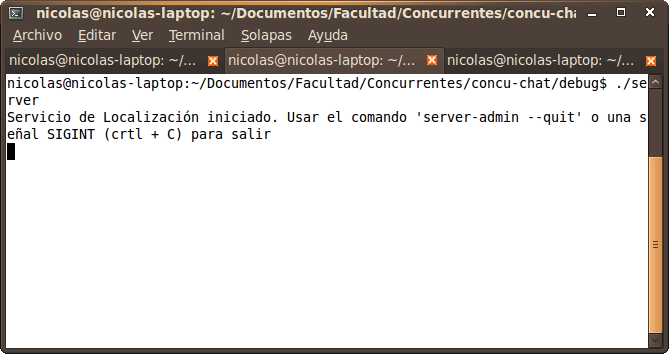
\includegraphics[scale=0.65]{./Images/Server}
\end{center}

\begin{itemize}
  \item Correr usuarios.
\end{itemize}
\begin{center}
  \small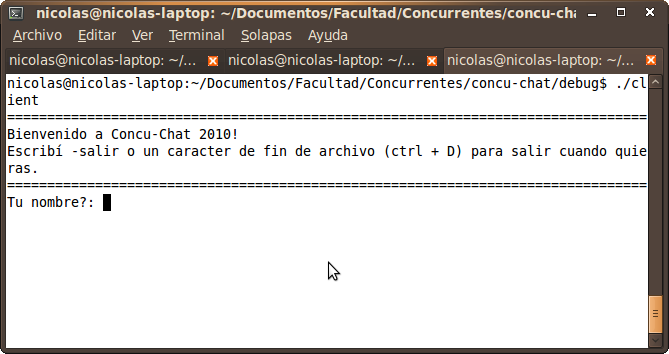
\includegraphics[scale=0.65]{./Images/Cliente}
\end{center}

\begin{itemize}
  \item Usuarios ingresan nombres.
\end{itemize}
\begin{center}
  \small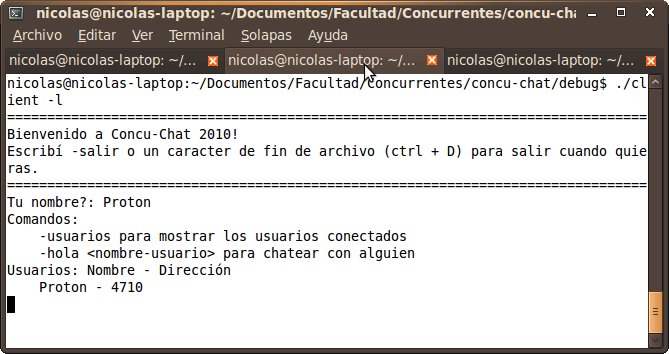
\includegraphics[scale=0.65]{./Images/Conver1}
  \small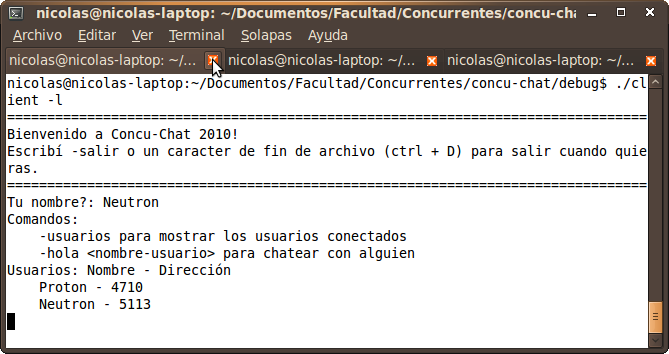
\includegraphics[scale=0.65]{./Images/Conver2}
\end{center}

\begin{itemize}
  \item Un usuario envia una petición de chat, y el otro la acepta.
\end{itemize}
\begin{center}
  \small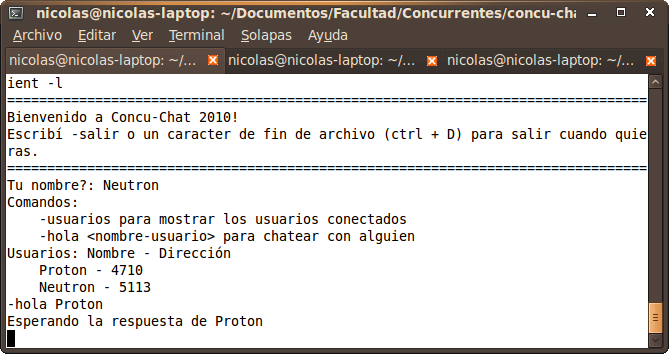
\includegraphics[scale=0.65]{./Images/Conver3}
  \small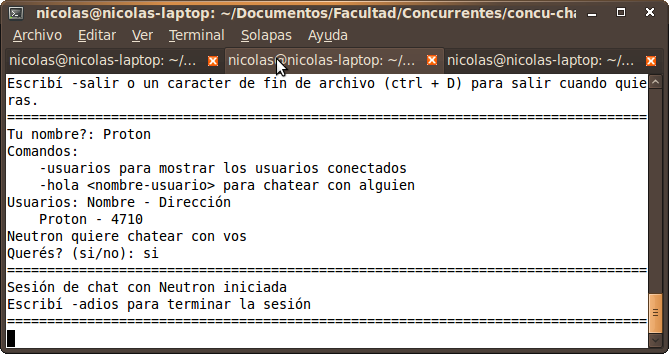
\includegraphics[scale=0.65]{./Images/Conver4}
\end{center}

\begin{itemize}
  \item Usuarios chateando.
\end{itemize}
\begin{center}
  \small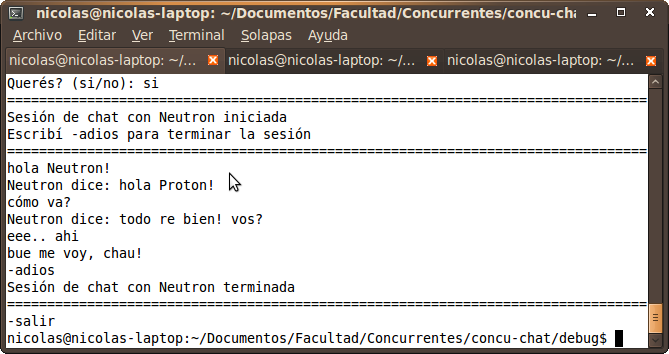
\includegraphics[scale=0.65]{./Images/Conver5}
  \small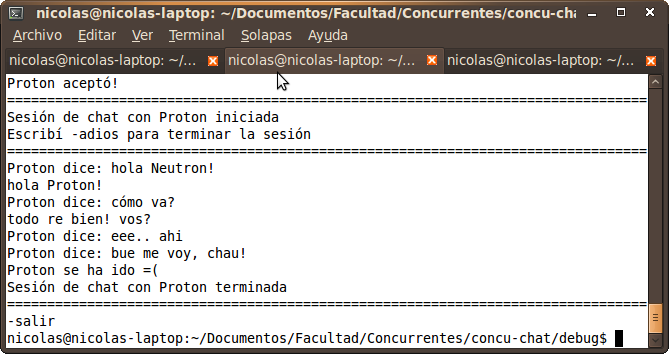
\includegraphics[scale=0.65]{./Images/Conver6}
\end{center}
